\documentclass{standalone}
\usepackage{tikz}
\begin{document}
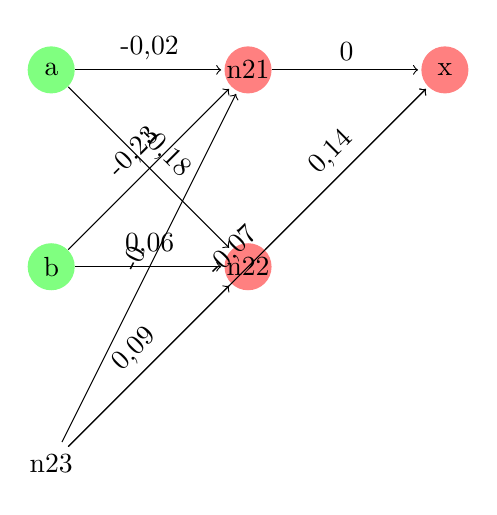
\begin{tikzpicture}[shorten >=1pt,->,draw=black!,node distance=2.5cm]
\tikzstyle{neuron}=[circle,fill=black!25,minimum size=17pt,inner sep=0pt]
\tikzstyle{constant}=[neuron, fill=white!50];
\tikzstyle{identity}=[neuron, fill=green!50];
\tikzstyle{sigmoid}=[neuron, fill=red!50];
\node [identity] (a) {a};
\node [identity,below of=a] (b) {b};
\node [constant,below of=b] (n23) {n23};
\node [sigmoid,right of=a] (n21) {n21};
\node [sigmoid,below of=n21] (n22) {n22};
\node [sigmoid,right of=n21] (x) {x};
\path[every node/.style={sloped,anchor=south,auto=false}]
(a) edge node {-0,18} (n22)
(a) edge node {-0,02} (n21)
(b) edge node {-0,23} (n21)
(b) edge node {0,06} (n22)
(n21) edge node {0} (x)
(n22) edge node {0,14} (x)
(n23) edge node {0,09} (n22)
(n23) edge node {-0,07} (x)
(n23) edge node {-0} (n21)
;\end{tikzpicture}
\end{document}